\documentclass[a4paper, 11pt]{article}
\usepackage{comment} % enables the use of multi-line comments (\ifx \fi) 
\usepackage{xparse}% http://ctan.org/pkg/xparse
\NewDocumentCommand{\Log}{o}{%
  \IfNoValueTF{#1}{}{{}^{#1}\!}\log}%
  
\usepackage{fullpage} % changes the margin
\usepackage{longtable}
\usepackage{graphicx}
\usepackage{fancyvrb,xcolor}
\usepackage{listings}
\usepackage{color}
\usepackage[hyphenbreaks]{breakurl}
\usepackage[hyphens]{url}
\usepackage[margin=3cm]{geometry}
\usepackage{relsize}
\definecolor{dkgreen}{rgb}{0,0.6,0}
\definecolor{gray}{rgb}{0.5,0.5,0.5}
\definecolor{mauve}{rgb}{0.58,0,0.82}
\usepackage{float}
\usepackage{caption}
\DeclareCaptionFont{white}{\color{white}}
\DeclareCaptionFormat{listing}{\colorbox{gray}{\parbox{\textwidth}{#1#2#3}}}
\captionsetup[lstlisting]{format=listing,labelfont=white,textfont=white}
\newcommand{\bigqm}[1][1]{\text{\larger[#1]{\textbf{?}}}}
\lstset{
  language=Java,
  aboveskip=3mm,
  belowskip=3mm,
  showstringspaces=false,
  columns=flexible,
  basicstyle={\small\ttfamily},
  numbers=none,
  numberstyle=\tiny\color{gray},
  keywordstyle=\color{blue},
  commentstyle=\color{dkgreen},
  stringstyle=\color{mauve},
  breaklines=true,
  breakatwhitespace=true,
  tabsize=3
}
\graphicspath{ {images/} }

\begin{document}
%Header-Make sure you update this information!!!!
\noindent
\large\textbf{Assignment 4} \hfill \textbf{Hussam Hallak} \\
\normalsize CS532, Web Science, Spring 2017\hfill CS Master's Student \\
Old Dominion University, Computer Science Dept \hfill Prof: Dr. Nelson 

\section*{Question 1:}
Determine if the friendship paradox holds for my Facebook
account.* Compute the mean, standard deviation, and median of the
number of friends that my friends have.  Create a graph of the
number of friends (y-axis) and the friends themselves, sorted by
number of friends (x-axis).  (The friends don't need to be labeled
on the x-axis: just f1, f2, f3, ... fn.)  Do include me in the graph
and label me accordingly.

* = This used to be more interesting when you could more easily download
your friend's friends data from Facebook.  Facebook now requires each
friend to approve this operation, effectively making it impossible.

I will email to the list the XML file that contains my Facebook
friendship graph ca. Oct, 2013.  The interesting part of the file looks
like this (for 1 friend):

\begin{lstlisting}
<node id="Johan_Bollen_1448621116">
        <data key="Label">Johan Bollen</data>
        <data key="uid"><![CDATA[1448621116]]></data>
        <data key="name"><![CDATA[Johan Bollen]]></data>
        <data key="mutual_friend_count"><![CDATA[37]]></data>
        <data key="friend_count"><![CDATA[420]]></data>
</node>
\end{lstlisting}

It is in GraphML format: http://graphml.graphdrawing.org/


\subsection*{Answer:}
I created a simple python program to parse the file ``mln.graphml'' and capture the number of friends for each friend of Dr. Nelson. These numbers are sorted and saved in a file named ``friendscount.txt'', which will be used later to generate the friendship paradox graph in R.

\lstinputlisting[language=Python, breakatwhitespace=〈false), label=parse.py, caption=The content of parse.py]{Q1/parse.py}

\begin{lstlisting}[language=bash, breakatwhitespace=〈false), label=running parse.py, caption= Running parse.py to capture the number of friends for each friend of Dr. Nelson]
root@ima-app:/var/www/Hussam/A4# python parse.py  mln.graphml
Total friends of friends of mln including his:
55284
mln friends count:
154
Mean:
359.0
Median:
266.5
STD:
370.4
\end{lstlisting}

The program created the output file and printed out the mean, standard deviation, and median of the number of friends that mln friends have. The number of Dr. Nelson's friends is not included in the calculations, but included in the output file to use it in the graph.

I wrote R code to create the graph of the number of friends (y-axis) and the friends themselves, sorted by number of friends (x-axis). The graph shows the position of Dr. Nelson among his friends colored in red on the graph and the mean value colored in blue.  

\begin{lstlisting}[language=R, breakatwhitespace=〈false), label=Friendship Paradox graph code in R, caption= Friendship Paradox graph code in R]
> friendcounts <- read.table("C:/R/friendscount.txt")
> mn <- 359
> mln <- 154
> cols = ifelse((friendcounts$V1 == mln), "red", (ifelse(abs(friendcounts$V1 == mn), "blue" , "orange")))
> barplot(friendcounts$V1, col= cols, border=cols, main="Friendship Paradox", xlab="Friends", ylab = "Number of Friends")
\end{lstlisting}

\begin{figure}[H]
\centering
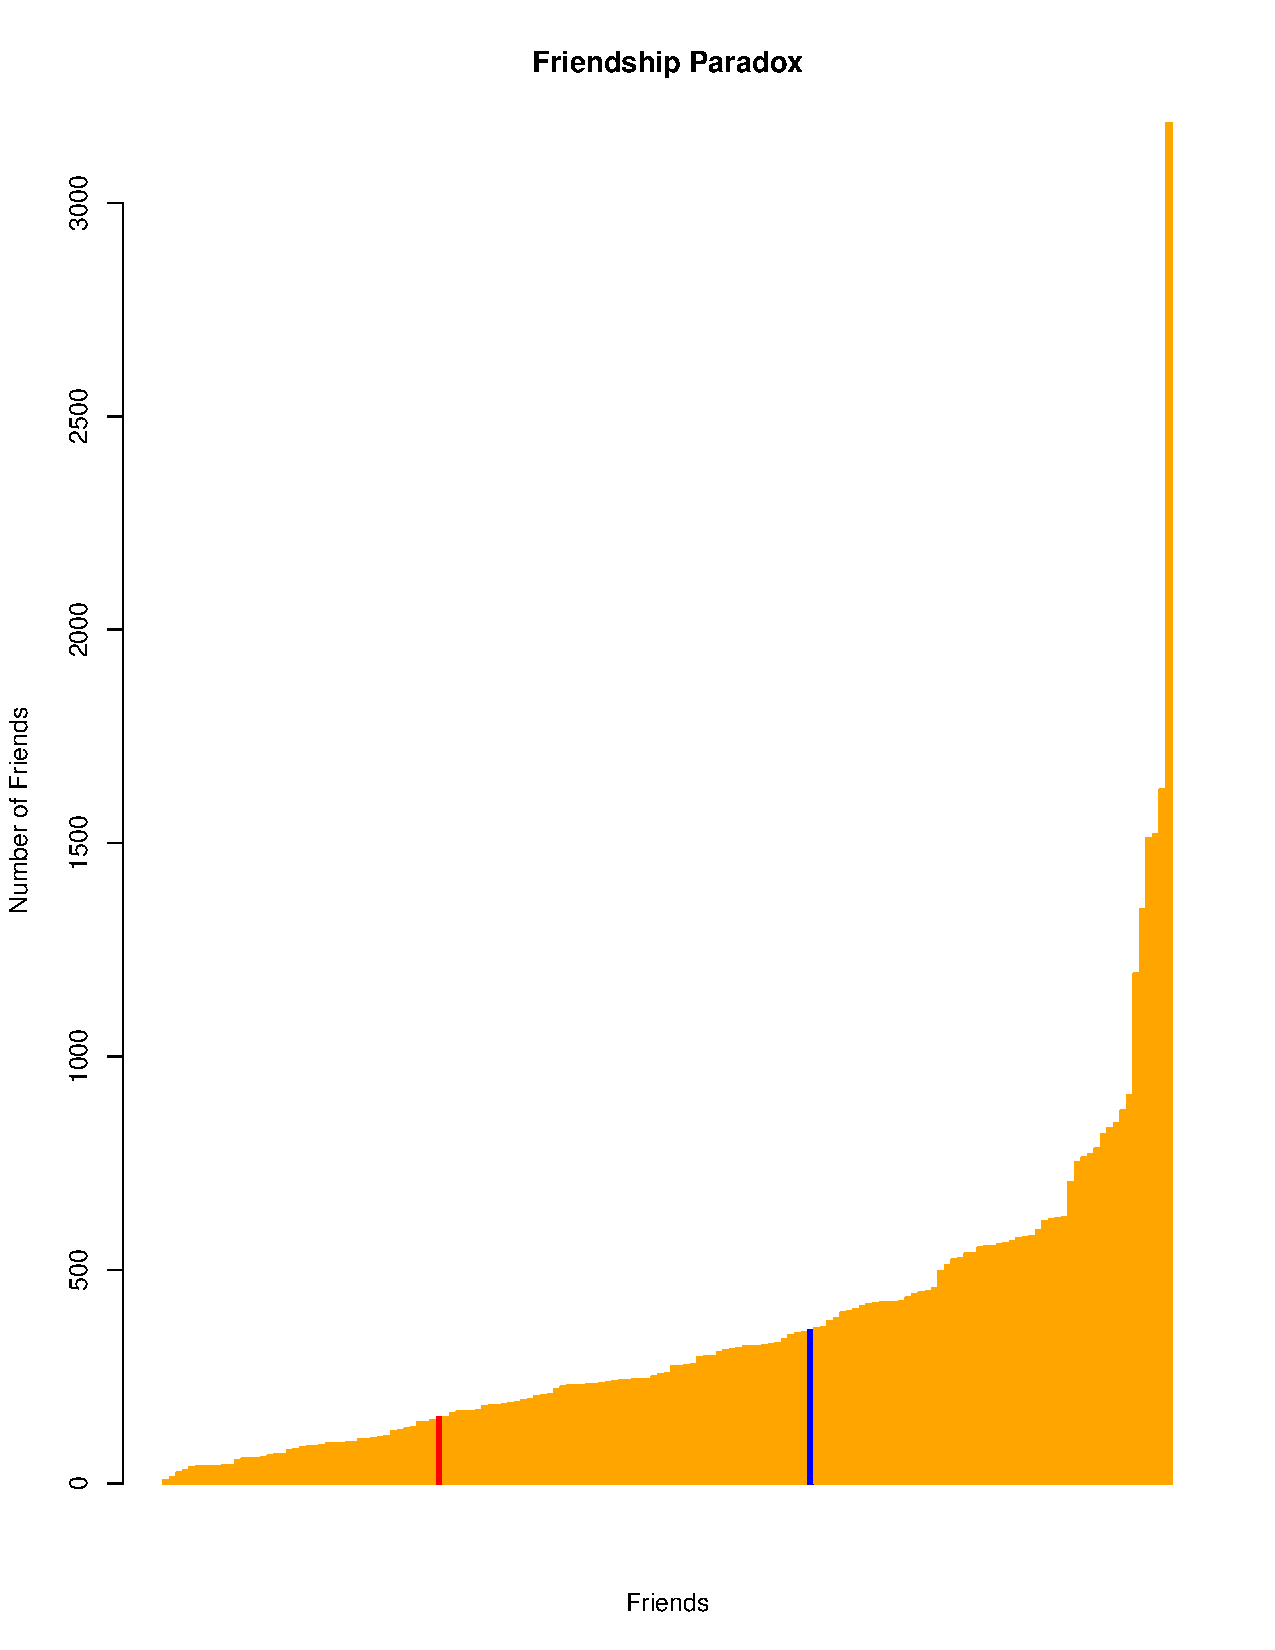
\includegraphics[scale=0.6]{facebook.pdf}
\end{figure}

Looking at the graph, it is obvious that the friendship paradox holds for Dr. Nelson’s account. His friends count is 154 and the mean is higher. The mean is 359.0 and the median is 266.5.


\subsection*{Included Files:}
parse.py, friendscount.txt, A4-1.Rproj, facebook.pdf, mln.graphml

\section*{Question 2:}
Determine if the friendship paradox holds for your Twitter account.
Since Twitter is a directed graph, use ``followers'' as value you measure
(i.e., ``do your followers have more followers than you?'').

Generate the same graph as in question \#1, and calculate the same 
mean, standard deviation, and median values.

For the Twitter 1.1 API to help gather this data, see:

https://dev.twitter.com/docs/api/1.1/get/followers/list

If you do not have followers on Twitter (or don't have more than 50),
then use my twitter account ``phonedude\_mln''.

\subsection*{Answer:}

I do not have a minimum of 50 followers on Twitter, so I used ``phonedude\_mln'' instead. I wrote a python program to capture the number of followers for users following ``phonedude\_mln''. The extracted data is saved to a file named ``followerscount.txt''.

\textbf{Note:}
Followers of ``phonedude\_mln'' that do not have any followers have been taken in consideration when calculating the mean, median, and standard deviation; however, they are not saved in the output file because 0 generates an error when creating the graph and setting the ``log'' argument to ``y'' because $log(0)$ is undefined and causes R to produce an error.

\lstinputlisting[language=Python, breakatwhitespace=〈false), label=parse.py, caption=The content of config.py]{Q2/config.py}

\lstinputlisting[language=Python, breakatwhitespace=〈false), label=getfollowersdata.py, caption=The content of getfollowersdata.py]{Q2/getfollowersdata.py}

\begin{lstlisting}[language=bash, breakatwhitespace=〈false), label=Running getfollowers.py, caption= Running getfollowersdata.py]
root@ima-app:/var/www/Hussam/A4# python getfollowersdata.py phonedude_mln
/usr/local/lib/python2.7/dist-packages/requests/packages/urllib3/util/ssl_.py:334: SNIMissingWarning: An HTTPS request has been made, but the SNI (Subject Name Indication) extension to TLS is not available on this platform. This may cause the server to present an incorrect TLS certificate, which can cause validation failures. You can upgrade to a newer version of Python to solve this. For more information, see https://urllib3.readthedocs.io/en/latest/advanced-usage.html#ssl-warnings
  SNIMissingWarning
/usr/local/lib/python2.7/dist-packages/requests/packages/urllib3/util/ssl_.py:132: InsecurePlatformWarning: A true SSLContext object is not available. This prevents urllib3 from configuring SSL appropriately and may cause certain SSL connections to fail. You can upgrade to a newer version of Python to solve this. For more information, see https://urllib3.readthedocs.io/en/latest/advanced-usage.html#ssl-warnings
  InsecurePlatformWarning
/usr/local/lib/python2.7/dist-packages/requests/packages/urllib3/util/ssl_.py:132: InsecurePlatformWarning: A true SSLContext object is not available. This prevents urllib3 from configuring SSL appropriately and may cause certain SSL connections to fail. You can upgrade to a newer version of Python to solve this. For more information, see https://urllib3.readthedocs.io/en/latest/advanced-usage.html#ssl-warnings
  InsecurePlatformWarning
Total followers of followers of  phonedude_mln  including his:
1017606
phonedude_mln 's followerss count:
634
Mean:
1605.1
Median:
311.5
STD:
10418.1
\end{lstlisting}

The program created the output file and printed out the mean, standard deviation, and median of the number of followers that ``phonedude\_mln' followers have. The number of Dr. Nelson's followers is not included in the calculations, but included in the output file to use it in the graph.

I wrote R code to create the graph of the number of followers (y-axis) and the followers themselves, sorted by number of followers (x-axis). The graph shows the position of Dr. Nelson among his followers colored in red on the graph and the mean value colored in blue.  

\begin{lstlisting}[language=R, breakatwhitespace=〈false), label=Followship Paradox graph code in R, caption= Followship Paradox graph code in R]
> followercounts <- read.table("C:/R/followerscount.txt")
> mn <- 1605.1
> mln <- 634
> cols = ifelse((followercounts$V1 == mln), "red", (ifelse((abs(followercounts$V1 - mn) < 21), "blue" , "orange")))
> barplot(followercounts$V1, col= cols, border=cols, main="Followship Paradox", xlab="Followers", ylab = "Number of Followers", log="y")
\end{lstlisting}

\begin{figure}[H]
\centering
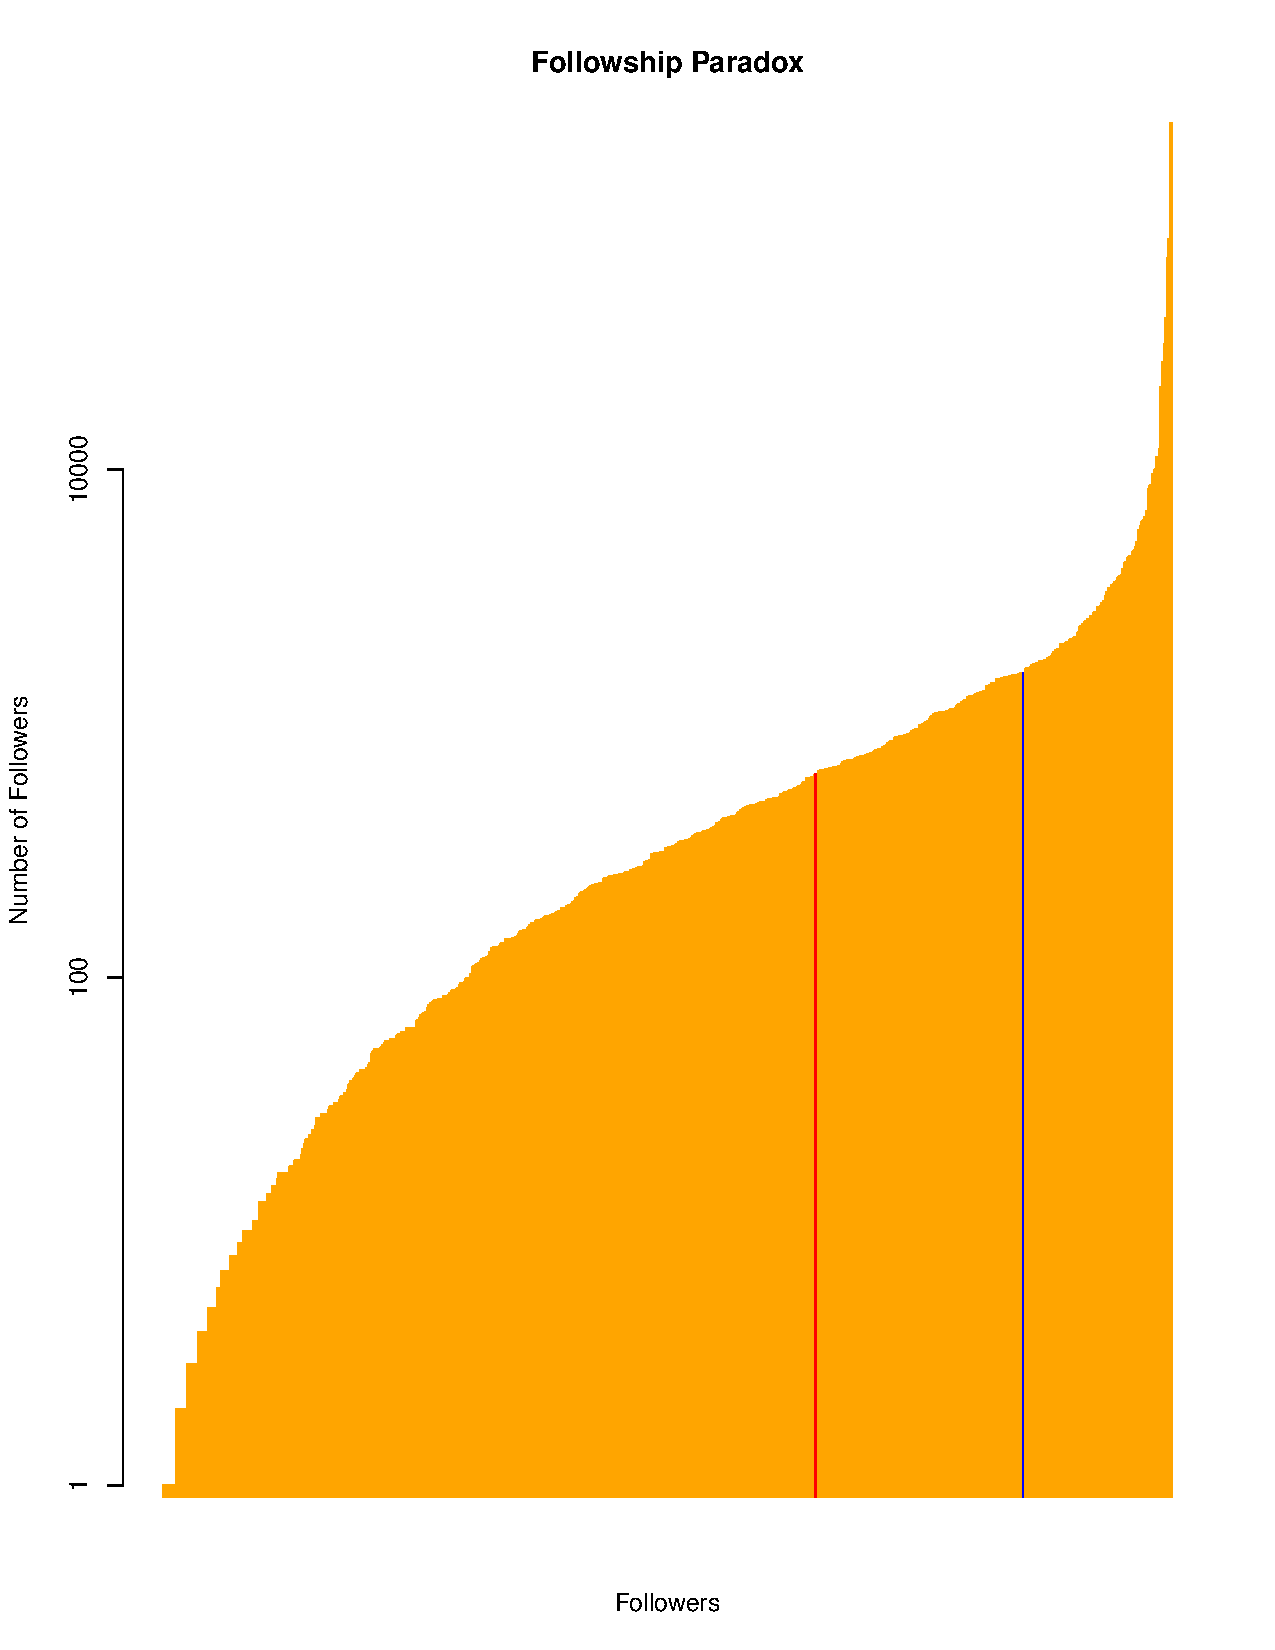
\includegraphics[scale=0.7]{twitter.pdf}
\end{figure}

Looking at the graph, it is obvious that the Followship Paradox holds for Dr. Nelson’s account. He has 634 followers and the mean is higher. The mean is 1605.1 and the median is 311.5.


\subsection*{Included Files:}
getfollowersdata.py, config.py followerscount.txt, A4-2.Rproj, twitter.pdf


\end{document}
